%\VignetteIndexEntry{Additional documentation of the function hhh4}
%\VignetteKeyword{getting started}
%\VignettePackage{surveillance}

\documentclass[a4paper,11pt]{article}
\usepackage{natbib}
\bibliographystyle{apalike}

% Preamble parts
\usepackage[T1]{fontenc}        % Make it possible to use danish characters !!
\usepackage[utf8]{inputenc}
\usepackage{url}
\usepackage{hyperref}
\usepackage{times}  
\renewcommand{\sfdefault}{ptm} 

\usepackage{bm}
\usepackage{amsmath}
\usepackage{amssymb}
\usepackage{latexsym}
\usepackage{verbatim}
\usepackage{relsize}
\usepackage{epsfig}
\usepackage{comment}

\usepackage{pdfpages}

\setlength{\parindent}{0pt} 
\setcounter{secnumdepth}{1}

\newcommand{\Po}{\operatorname{Po}}
\newcommand{\NegBin}{\operatorname{NegBin}}
\newcommand{\n}{{\cal N}}

\newcommand{\surveillance}{\texttt{surveillance}}
\newcommand{\code}[1]{\texttt{#1}}
\newcommand{\hhh}{\texttt{hhh4}}
\newcommand{\R}{\textsf{R}}
\newcommand{\sts}{\texttt{sts}}
\newcommand{\example}[1]{\textit{Example: #1}}

\title{The function `hhh4' in the R-package `surveillance'}  %'
\author{
Michaela Paul\thanks{Author of correspondence: Email: \texttt{michaela.paul@ifspm.uzh.ch}}\\
Biostatistics Unit\\
Institute of Social and Preventive Medicine\\
University of Zurich, Switzerland
} 
\date{\today}

\usepackage{Sweave}
\begin{document}
%%%%%%%%%%%%%%%%%%%%%%%%%%%%%%%%%%%%%%%%%%%%%%%%%%%%%%%%%%%%%%%%%%%%%%
% Sweave 
%%%%%%%%%%%%%%%%%%%%%%%%%%%%%%%%%%%%%%%%%%%%%%%%%%%%%%%%%%%%%%%%%%%%%%

\setkeys{Gin}{width=1\textwidth} 

\definecolor{Sinput}{rgb}{0,0,0.56}
\definecolor{Scode}{rgb}{0,0,0.56}
\definecolor{Soutput}{rgb}{0,0,0}

\DefineVerbatimEnvironment{Sinput}{Verbatim}{formatcom={\color{Sinput}},fontshape=sl,fontsize=\relsize{-1}}
\DefineVerbatimEnvironment{Soutput}{Verbatim}{formatcom={\color{Soutput}},fontfamily=courier, fontshape=it,fontsize=\relsize{-2}}
\DefineVerbatimEnvironment{Scode}{Verbatim}{formatcom={\color{Scode}},fontshape=sl,fontsize=\relsize{-1}}


%%%%%%%%%%%%%%%%%%%%%%%%%%%%%%%%%%%%%%%%%%%%%%%%%%%%%%%%%%%%%%%%%%%%%%
% Initial R code
%%%%%%%%%%%%%%%%%%%%%%%%%%%%%%%%%%%%%%%%%%%%%%%%%%%%%%%%%%%%%%%%%%%%%%




\maketitle  

\begin{abstract}
  \noindent This document gives an introduction to the use of the function 
  \hhh\ for modelling univariate and multivariate time series of infectious 
  disease counts. The function is part of the \R-package \surveillance, 
  which provides tools for the visualization, modelling and monitoring of 
  surveillance time series. 
  The basic functionality of \surveillance\ is introduced in 
  the package vignette \citep{vignette} and in \cite{hoehle-2007} with main 
  focus on outbreak detection methods. The following illustrates the use 
  of \hhh\ as estimation and prediction routine for the modelling framework 
  proposed by \citet{held-etal-2005}, and extended in \citet{paul-etal-2008}, 
  \citet{paul-held-2011} and \citet{herzog-etal-2010}.
\end{abstract}


\section{Introduction}\label{sec:intro}

To meet the threats of infectious diseases, many countries have established
surveillance systems for the reporting of various infectious diseases.
The systematic and standardized reporting at a national and regional level 
aims to recognize all outbreaks quickly, even when aberrant cases are 
dispersed in space. Traditionally, notification data, i.e.\ counts of cases 
confirmed according to a specific definition and reported daily, weekly or 
monthly on a regional or national level, are used for surveillance purposes.

The \R-package \surveillance\ provides functionality for the retrospective 
modelling and prospective change-point detection in the resulting surveillance 
time series. A recent introduction to the package with focus on outbreak 
detection methods is given by \cite{hoehle-mazick-2010}.

This document illustrates the functionality of the function \hhh\
for the modelling of univariate and multivariate time series 
of infectious disease counts. 
The function is currently incorporated in the development version of 
\surveillance\ available from \url{http://surveillance.r-forge.r-project.org/}.
Section~\ref{sec:data} introduces the S4 class data structure used to store 
surveillance time series data within the package. Access and 
visualization methods are outlined by means of built-in data sets.
In Section~\ref{sec:model}, the statistical modelling approach by 
\cite{held-etal-2005} and further model extensions are described. 
After the general function call and arguments 
are shown, the detailed usage of \hhh\ is demonstrated in 
Section~\ref{sec:hhh} using data introduced in Section~\ref{sec:data}. 

%%%%%%%%%%%%%%%%%%%%%%%%%%%%%%%%%%%%%%%%%%%%%%%%%%%%%%%%%%%%%%%%%%%%%%%%%%
%%  DATA
%%%%%%%%%%%%%%%%%%%%%%%%%%%%%%%%%%%%%%%%%%%%%%%%%%%%%%%%%%%%%%%%%%%%%%%%%%
\section{Surveillance data}\label{sec:data}

Denote by $\{y_{it}; i=1,\ldots,I,t=1,\ldots,T\}$ the multivariate time series
of disease counts for a specific partition of gender, age and location. 
Here, $T$ denotes the length of the time series and $I$ denotes the number 
of units (e.g\ geographical regions or age groups) being monitored.
Such data are represented using objects of the S4 class \sts\ (surveillance 
time series).

This class contains the $T\times I$ matrix of counts $y_{it}$ in
a slot \code{observed}. An integer slot \code{epoch} denotes the time index
$1\leq t \leq T$ of each row in \code{observed}. The number of observations
per year, e.g.\ 52 for weekly or 12 for monthly data, is denoted by \code{freq}.
Furthermore, \code{start} denotes a vector of length two containing the start
of the time series as \code{c(year, epoch)}.
For spatially stratified time series, the slot \code{neighbourhood}
denotes an $I \times I$ adjacency matrix with elements 1 if two regions are
neighbors and 0 otherwise. For map visualizations, the slot \code{map} 
links the multivariate time series to geographical regions of an ESRI shapefile
(using functionality from the package \code{maptools}~\citep{maptools}).
Additionally, the slot \code{populationFrac} contains a $T\times I$ matrix
representing population fractions in unit $i$ at time $t$.


The package \surveillance\ contains a number of time series in the \code{data}
directory. Most data sets originate from the SurvStat@RKI database 
(\url{http://www3.rki.de/SurvStat}), maintained by the Robert Koch Institute 
(RKI), Germany. Selected data sets will be analyzed in Section~\ref{sec:hhh} 
and are introduced in the following. Note that many of the built-in datasets 
are stored in the S3 class data structure \code{disProg}. 
They can be easily converted into the S4 \sts\ data structure using
the function \code{disProg2sts}. The resulting \sts\ object can be accessed 
similar as standard \code{matrix} objects and allows easy temporal and spatial
aggregation as will be shown in the remainder of this section. \\

%%%%%%%%%%%%%%%%%%%%%%%%%%%%%%%%%%%%%%%%%%%%%%%%%%%%%%%%%%%%%%%%%%%%%
\example{Influenza and meningococcal disease in Germany 01/2001--52/2006}
%%%%%%%%%%%%%%%%%%%%%%%%%%%%%%%%%%%%%%%%%%%%%%%%%%%%%%%%%%%%%%%%%%%%%

As a first example, the weekly number of influenza and meningococcal disease 
cases in Germany is considered.
\begin{Schunk}
\begin{Sinput}
> # load data
> data("influMen")
> # convert to sts class and print basic information about the time series
> print(fluMen <- disProg2sts(influMen))
\end{Sinput}
\begin{Soutput}
-- An object of class sts -- 
freq:		 52 
start:		 2001 1 
dim(observed):	 312 2 

Head of observed:
     influenza meningococcus
[1,]         7             4

map:
NULL

head of neighbourhood:
          influenza meningococcus
influenza         0             1
\end{Soutput}
\end{Schunk}
The univariate time series of meningococcal disease counts can be obtained
with
\begin{Schunk}
\begin{Sinput}
> meningo <- fluMen[, "meningococcus"]
> dim(meningo)
\end{Sinput}
\begin{Soutput}
[1] 312   1
\end{Soutput}
\end{Schunk}
The \code{plot} function provides an interface to the visual representation
of the multivariate time series in time, space and space-time which is
controlled by the \code{type} argument:
\begin{Schunk}
\begin{Sinput}
> plot(fluMen, type = observed ~ time | unit, # type of plot
+              same.scale = FALSE,            # unit-specific ylim ?
+              col = "grey"                   # color of bars
+              )
\end{Sinput}
\end{Schunk}
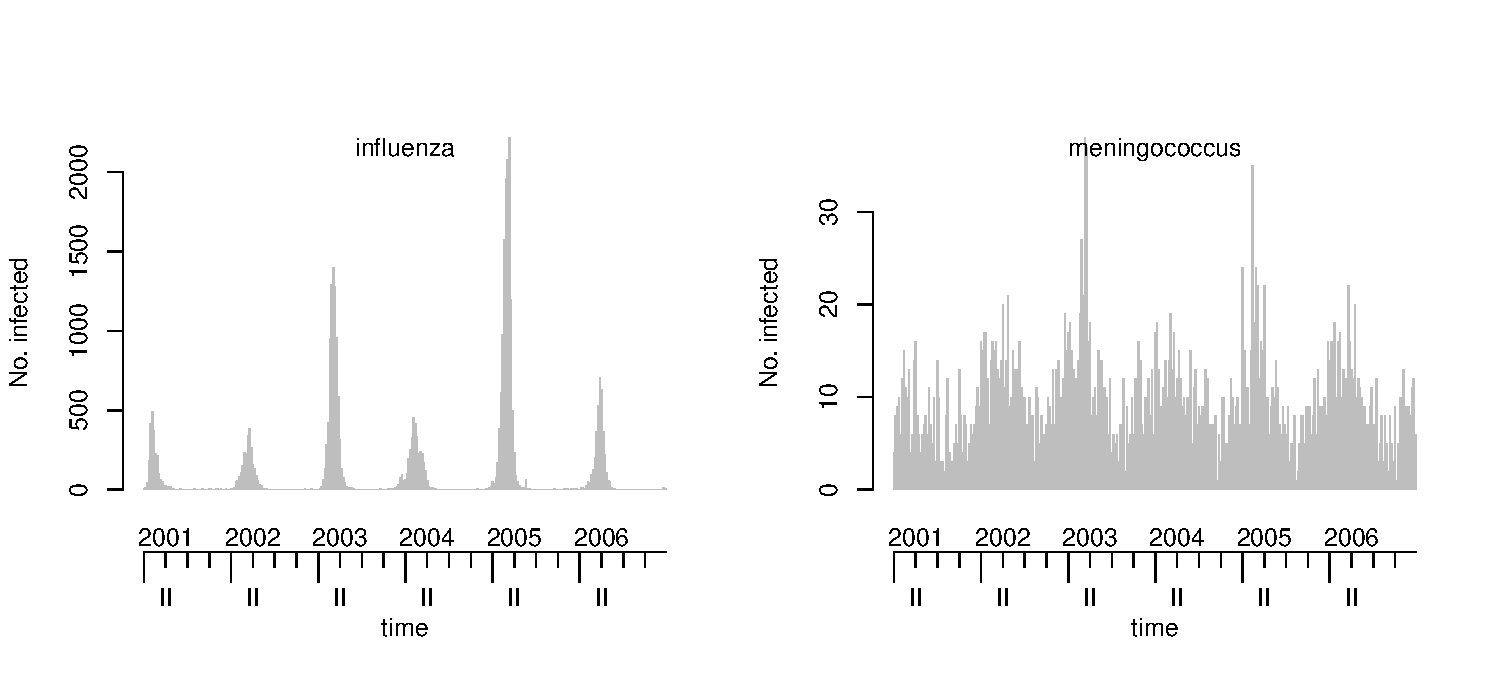
\includegraphics{figs/vignette_hhh4-fluMen}
See \cite{hoehle-mazick-2010} for a detailed description of the plot routines.\\


%%%%%%%%%%%%%%%%%%%%%%%%%%%%%%%%%%%%%%%%%%%%%%%%%%%%%%%%%%%%%%%%%%%%%%%
\example{Influenza in Southern Germany, 01/2001-52/2008}
%%%%%%%%%%%%%%%%%%%%%%%%%%%%%%%%%%%%%%%%%%%%%%%%%%%%%%%%%%%%%%%%%%%%%%%
The spatio-temporal spread of influenza in the 140 Kreise (districts) 
of Bavaria and Baden-W\"urttemberg  is analyzed using the weekly number of 
cases reported to the RKI~\citep{survstat-fluByBw} in the years 2001--2008.
An \sts\ object containing the data is created as follows:
\begin{Schunk}
\begin{Sinput}
> # read in observed number of cases
> flu.counts <- as.matrix(read.table(system.file("extdata/counts_flu_BYBW.txt", 
+                                       package = "surveillance")))
> # remove 'X' in column names                                      
> colnames(flu.counts) <- substring(colnames(flu.counts),first = 2, last = 5)                                      
> # read in adjacency matrix with elements 1 if two regions share a common border
> nhood <- as.matrix(read.table(system.file("extdata/neighbourhood_BYBW.txt",
+                                       package = "surveillance")))
> # visualize adjacency matrix
> image(Matrix(nhood))
\end{Sinput}
\end{Schunk}
\begin{center}
\vspace*{-2em}
\setkeys{Gin}{width=.5\textwidth}
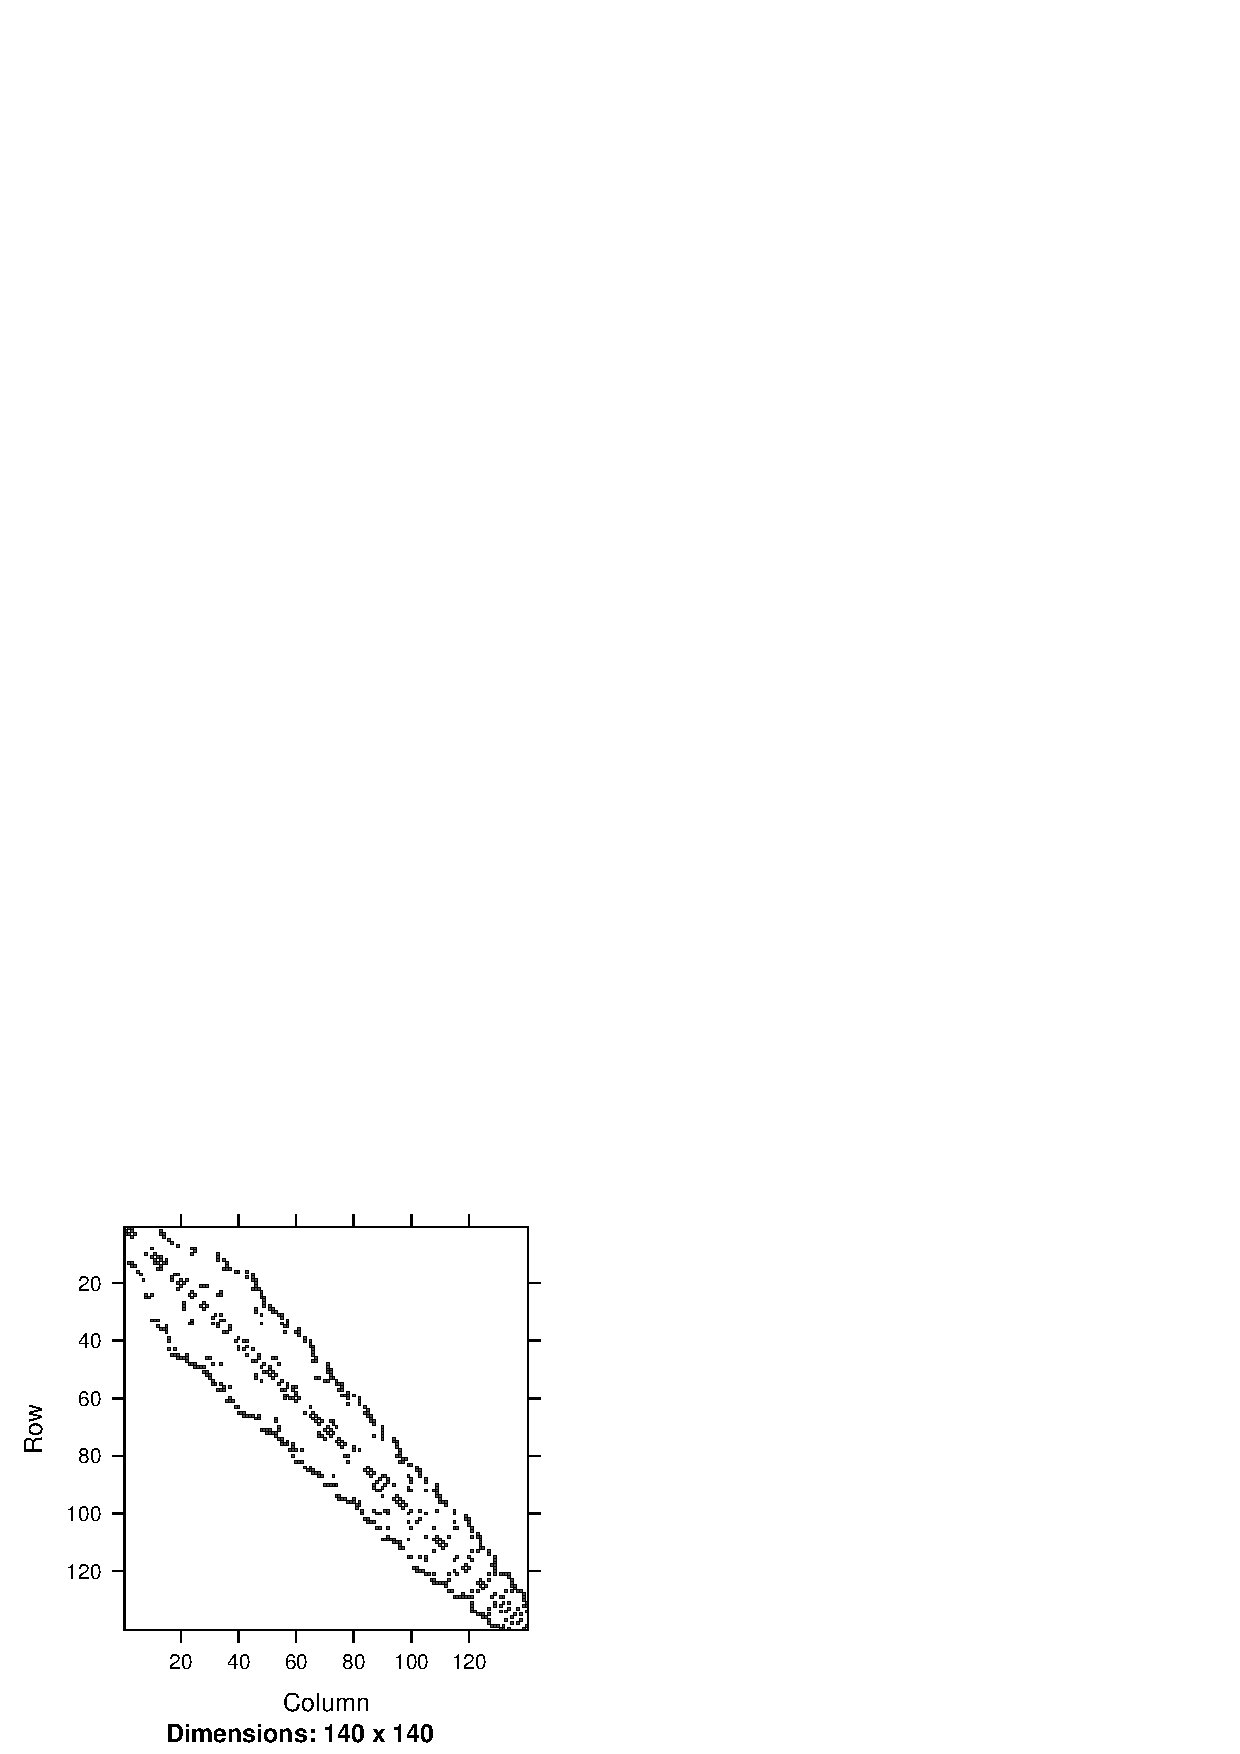
\includegraphics{figs/vignette_hhh4-nhoodByBw}
\end{center}
\begin{Schunk}
\begin{Sinput}
> # read in a shapefile of the districts in Bavaria and Baden-Wuerttemberg
> map <- readShapePoly(system.file("shapes/districts_BYBW.shp",
+                         package = "surveillance"), IDvar = "id")
> # read in population fractions
> p <- matrix(read.table(system.file("extdata/population_2001-12-31_BYBW.txt",
+                           package = "surveillance"), header = TRUE)$popFrac, 
+             nrow = nrow(flu.counts), ncol= ncol(flu.counts), byrow = TRUE)
> # create sts object
> flu <- new("sts", epoch = 1:nrow(flu.counts),
+                   observed = flu.counts,
+                   start = c(2001, 1),
+                   freq = 52,
+                   neighbourhood = nhood,
+                   map = map,
+                   population = p
+                   )
\end{Sinput}
\end{Schunk}
This \sts\ object is already included in \surveillance\ and may be
loaded with \code{data(fluBYBW)}.

A map of the total number of cases in the year 2001 may be obtained as follows:
\setkeys{Gin}{width=.5\textwidth}
%\vspace*{-2em}
\begin{center}
\begin{Schunk}
\begin{Sinput}
> par(mar=c(0,0,0,0))
> plot(flu[year(flu) == 2001, ],    # select year 2001
+      type = observed ~ 1 | unit,  # map of counts aggregated over times t
+      labels = FALSE               # suppress region labels in map
+      )
\end{Sinput}
\end{Schunk}
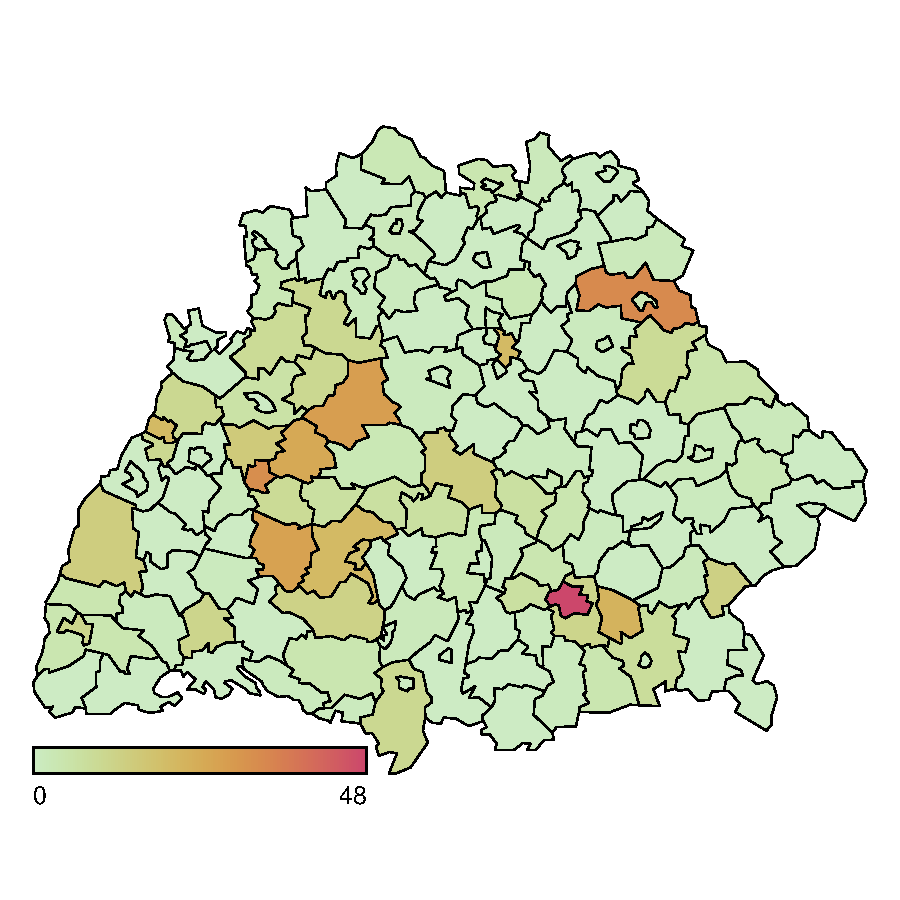
\includegraphics{figs/vignette_hhh4-flu-ByBw}
\end{center}

%%%%%%%%%%%%%%%%%%%%%%%%%%%%%%%%%%%%%%%%%%%%%%%%%%%%%%%%%%%%
\example{Measles in Germany, 01/2005--52/2007}
%%%%%%%%%%%%%%%%%%%%%%%%%%%%%%%%%%%%%%%%%%%%%%%%%%%%%%%%%%%%
The following data set contains the weekly number of measles cases in the 16
German Bundesl\"ander (federal states), in the years 2005--2007. These data 
are analyzed in~\cite{herzog-etal-2010} after aggregation into successive 
bi-weekly periods.

\setkeys{Gin}{width=1\textwidth}
\begin{center}
\begin{Schunk}
\begin{Sinput}
> data("measlesDE")
> # aggregate into successive bi-weekly periods
> measles2w <- aggregate(measlesDE, nfreq = 26)
> plot(measles2w, type = observed ~ time,   # plot aggregated over all units i
+                    main = "Bi-weekly number of measles cases in Germany", 
+                    legend.opts = NULL        # suppress default legend
+                    )
\end{Sinput}
\end{Schunk}
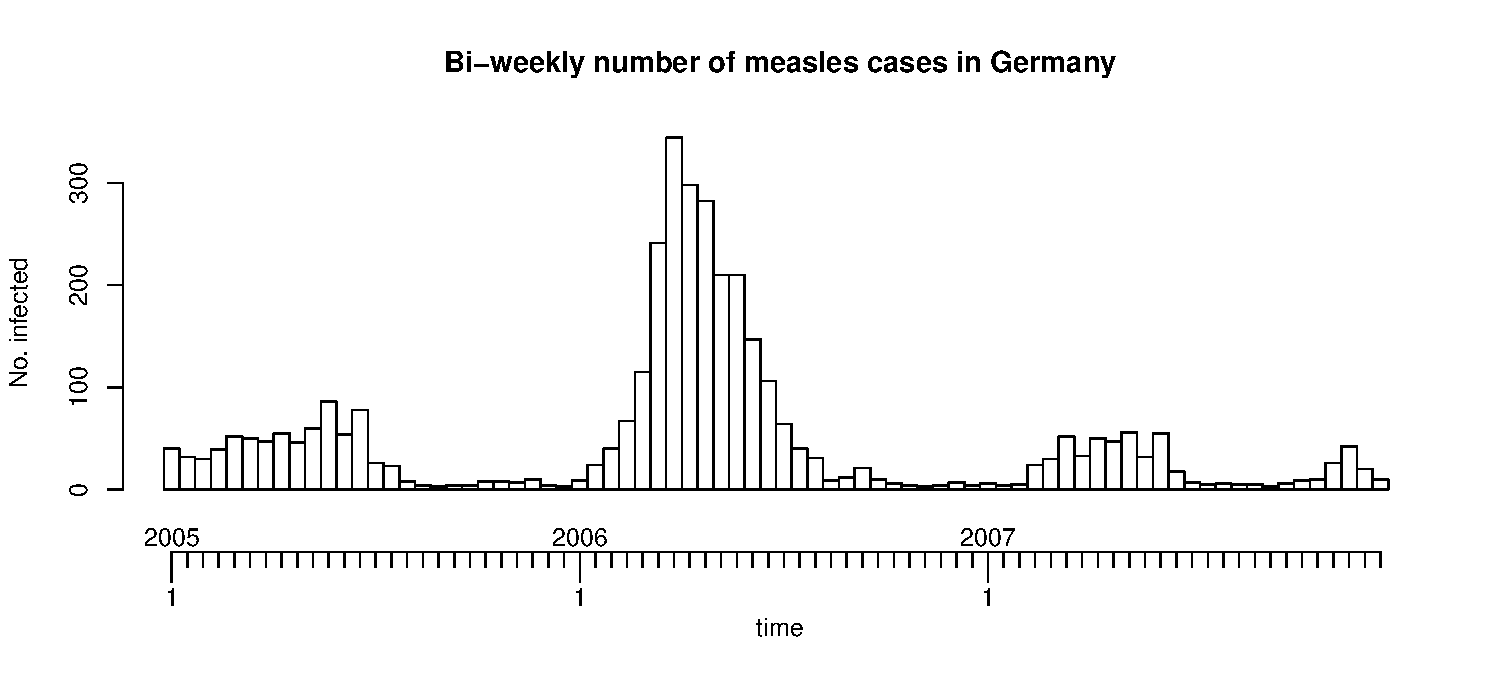
\includegraphics{figs/vignette_hhh4-measles}
\end{center}

%%%%%%%%%%%%%%%%%%%%%%%%%%%%%%%%%%%%%%%%%%%%%%%%%%%%%%%%%%%%%%%%%%%%
%% Model
%%%%%%%%%%%%%%%%%%%%%%%%%%%%%%%%%%%%%%%%%%%%%%%%%%%%%%%%%%%%%%%%%%%%
\section{Model formulation}\label{sec:model}

Retrospective surveillance aims to identify outbreaks and (spatio-)temporal
patterns through statistical modelling. Motivated by a branching process
with immigration, \cite{held-etal-2005} suggest the following model
for the analysis of univariate time series of infectious disease counts 
$\{y_{t}; t=1,\ldots,T\}$.
The counts are assumed to be Poisson distributed with conditional mean
\begin{align*}
  \mu_{t} = \lambda y_{t-1}+ \nu_{t}, \quad(\lambda,\nu_{t}>0)
\end{align*}
where $\lambda$ and $\nu_t$ are unknown quantities.
The mean incidence is decomposed additively into two components: an
epidemic or \emph{autoregressive} component $\lambda y_{t-1}$, and
an \emph{endemic} component $\nu_t$. The former should be able to capture
occasional outbreaks whereas the latter explains a baseline rate of cases
with stable temporal pattern. 
\cite{held-etal-2005} suggest the following parametric model for the endemic 
component:
\begin{align}\label{eq:nu_t}
  \log(\nu_t) =\alpha + \beta t +
              \left\{\sum_{s=1}^S \gamma_s \sin(\omega_s t) + \delta_s \cos(\omega_s t)\right\},
\end{align}
where $\alpha$ is an intercept, $\beta$ is a trend parameter, and the terms
in curly brackets are used to model seasonal variation. Here, $\gamma_s$ and
$\delta_s$ are unknown parameters, $S$ denotes the number of harmonics to 
include, and $\omega_s=2\pi s/$\code{freq} are Fourier frequencies (e.g.\
\code{freq = 52} for weekly data).
For ease of interpretation, the seasonal terms in \eqref{eq:nu_t} can be
written equivalently as 
\begin{align*}
 \gamma_s \sin(\omega_s t) + \delta_s \cos(\omega_s t)= A_s \sin(\omega_s t +\varphi_s)
\end{align*}
with amplitude $A_s=\sqrt{\gamma_s^2+\delta_s^2}$
describing the magnitude, and phase difference $\tan(\varphi_s)=\delta_s/\gamma_s$ 
describing the onset of the sine wave.

To account for overdispersion, the Poisson model may be replaced by
a negative binomial model. Then, the conditional mean $\mu_t$ remains
the same but the conditional variance increases to $\mu_t (1+\mu_t/\psi)$
with additional unknown overdispersion parameter $\psi>0$.

The model is extended to multivariate time series $\{y_{it}\}$ in 
\cite{held-etal-2005} and \cite{paul-etal-2008} by including an additional 
\emph{neighbor-driven} component, where past cases in other (neighboring) 
units also enter as explanatory covariates. The conditional mean $\mu_{it}$ 
is then given by
\begin{align} \label{eq:mu_it}
  \mu_{it} = \lambda y_{i,t-1} + \phi \sum_{j\neq i} w_{ji} y_{j,t-1} +e_{it} \nu_{t},
\end{align}
where the unknown parameter $\phi$ quantifies the influence of other units $j$ 
on unit $i$, $w_{ji}$ are suitably chosen known weights and $e_{it}$
corresponds to an offset (such as population fractions at time $t$ in region $i$).
A simple choice for the weights is $w_{ji}=1$ if units $j$ and $i$ are adjacent
and 0 otherwise. See \cite{paul-etal-2008} for a discussion of alternative
weights.

When analyzing a specific disease observed in, say, multiple regions or several
pathogens (such as influenza and meningococcal disease), the assumption
of equal incidence levels or disease transmission across units is
questionable. To address such heterogeneity, the unknown quantities
$\lambda$, $\phi$, and $\nu_t$ in \eqref{eq:mu_it} may also depend on unit
$i$. This can be done via
\begin{itemize}
  \item unit-specific fixed parameters, e.g.\ $\log(\lambda_i)=\alpha_i$ 
     \citep{paul-etal-2008};
  \item unit-specific random effects, e.g\ $\log(\lambda_i)=\alpha_0 +a_i$, 
     $a_i \stackrel{\text{iid}}{\sim} \n(0,\sigma^2_\lambda)$ \citep{paul-held-2011};
  \item linking parameters with known (possibly time-varying) explanatory 
     variables, e.g.\ $\log(\lambda_i)=\alpha_0 +x_i\alpha_1$ with
     region-specific vaccination coverage $x_i$ \citep{herzog-etal-2010}.
\end{itemize}

A call to \hhh\ fits a Poisson or negative binomial model with conditional
mean
\begin{align*}
  \mu_{it} = \lambda_{it} y_{i,t-1} + \phi_{it} \sum_{j\neq i} w_{ji} y_{j,t-1} +e_{it} \nu_{it}
\end{align*}
to a multivariate time series of counts.
Here, the three unknown quantities are decomposed additively on the log scale
\begin{align}
  \log(\lambda_{it}) &= \alpha_0 + a_i +\bm{u}_{it}^\top \bm{\alpha} \tag{\code{ar}}\\
  \log(\phi_{it}) &=  \beta_0 + b_i +\bm{x}_{it}^\top \bm{\beta} \tag{\code{ne}}\\
  \log(\nu_{it}) &=  \gamma_0 + c_i +\bm{z}_{it}^\top \bm{\gamma}\tag{\code{end}}
\end{align}
where $\alpha_0,\beta_0,\gamma_0$ are intercepts, $\bm{\alpha},\bm{\beta},\bm{\gamma}$
are vectors of unknown parameters corresponding to covariate vectors 
$\bm{u}_{it},\bm{x}_{it},\bm{z}_{it}$, and $a_i,b_i,c_i$ are random effects. 
For instance, model~\eqref{eq:nu_t} with $S=1$ seasonal terms may be
represented as $\bm{z}_{it}=(t,\sin(2\pi/\code{freq}\;t),\cos(2\pi/\code{freq}\;t))^\top$.
The stacked vector of all random effects
is assumed to follow a normal distribution with mean $\bm{0}$ and covariance
matrix $\bm{\Sigma}$, see \cite{paul-held-2011} for further details.
Inference is based on (penalized) likelihood methodology as proposed in 
\cite{paul-held-2011}. In applications, each component (\code{ar})--(\code{end}) 
may be omitted in parts or as a whole.


%%%%%%%%%%%%%%%%%%%%%%%%%%%%%%%%%%%%%%%%%%%%%%%%%%%%%%%%%%%%%%%%%%%%
%% Function call and arguments
%%%%%%%%%%%%%%%%%%%%%%%%%%%%%%%%%%%%%%%%%%%%%%%%%%%%%%%%%%%%%%%%%%%%
\section{Function call and control settings}\label{sec:hhh}

The estimation procedure is called with
\begin{Schunk}
\begin{Sinput}
> hhh4(sts, control)
\end{Sinput}
\end{Schunk}
where \code{sts} denotes a (multivariate) surveillance time series and
the model is specified in the argument \code{control} in consistency
with other algorithms in \surveillance.
The \code{control} setting is a list of the following arguments:

\begin{Schunk}
\begin{Sinput}
> control = list(
+     ar = list(f = ~ -1),       # formula: exp(u'alpha) * y_i,t-1 
+     ne = list(f = ~ -1,        # formula: exp(x'beta) * sum_j {w_ji * y_j,t-1} 
+               weights = NULL   # matrix with weights w_ji 
+                                # [w_ji = neighbourhood(stsObj) as default]
+               ),              
+     end = list(f = ~ 1,        # formula:  exp(z'gamma) * e_it 
+               offset = NULL    # optional offset e_it 
+               ),
+     family = "Poisson",                # Poisson or NegBin model
+     subset = 2:nrow(stsObj),           # subset of observations to be used 
+                                        # in the fitting process
+     optimizer = list(tech = "nlminb"), # details for optimizer 
+     verbose = FALSE,                   # no progress information is printed
+     start = list(fixed = NULL,         # list with initial values for fixed,
+                  random = NULL,        # random, and
+                  sd.corr = NULL        # variance parameters
+                  ),
+     data = data.frame(t = epoch(sts))  # data.frame,
+                                        # or named list with covariates 
+     )
>            
\end{Sinput}
\end{Schunk}
The first three arguments \code{ar}, \code{ne}, and \code{end} 
specify the model components using \code{formula} objects.
As default, the counts $y_{it}$ are assumed to be Poisson distributed.
A negative binomial model is obtained with \code{family = "NegBin1"}.
The log-likelihood is maximized using the optimization routine implemented
in \code{nlminb}. Alternatively, the methods implemented in
\code{optim} may be used, e.g.\ \code{optimizer = list(tech = "BFGS")}.
Initial values for the fixed, random, and variance parameters 
are passed on in the \code{start} argument.
If the model contains covariates, these have to be specified in the \code{data} 
argument. When covariates do not vary across units, they may be passed on as a 
vector of length $T$. Otherwise, covariate values have to be stored and passed on
in a matrix of size $T \times I$.


In the following, the functionality of \hhh\ is demonstrated using
the data sets introduced in Section~\ref{sec:data}
and previously analyzed in \cite{paul-etal-2008}, \cite{paul-held-2011} and 
\cite{herzog-etal-2010}.
Selected results are reproduced. For a thorough discussion 
we refer to these papers.

%%%%%%%%%%%%%%%%%%%%%%%%%%%%%%%%%%%%%%%%%%%%%%%%%%%%%%%%%%%%%%%%%%%%
\subsubsection{Univariate modelling}
%%%%%%%%%%%%%%%%%%%%%%%%%%%%%%%%%%%%%%%%%%%%%%%%%%%%%%%%%%%%%%%%%%%%

As a first example, consider the univariate time series of meningococcal infections
in Germany, 01/2001--52/2006 \citep[cf.~Tab.~1 in ][]{paul-etal-2008}.
A Poisson model without autoregression and $S=1$ seasonal term is specified 
as follows:
\begin{Schunk}
\begin{Sinput}
> # specify formula object for endemic component
> ( f_S1 <- addSeason2formula(f = ~ 1, S = 1, period = 52) )
\end{Sinput}
\begin{Soutput}
~1 + sin(2 * pi * t/52) + cos(2 * pi * t/52)
<environment: 0x605ebc8>
\end{Soutput}
\begin{Sinput}
> # fit Poisson model
> summary(hhh4(meningo, control = list(end = list(f = f_S1), family = "Poisson")))
\end{Sinput}
\begin{Soutput}
Call: 
hhh4(stsObj = meningo, control = list(end = list(f = f_S1), family = "Poisson"))


Fixed effects: 
                        Estimates  Std.Error
end.1                      2.2648     0.0187
end.sin(2 * pi * t/52)     0.3619     0.0259
end.cos(2 * pi * t/52)     0.2605     0.0258

log-likelihood:    -872.09 
AIC:               1750.19 
BIC:               1761.41 

Number of units:          1 
Number of time points:    311 
\end{Soutput}
\end{Schunk}
A corresponding negative binomial model is obtained via
\begin{Schunk}
\begin{Sinput}
> result1 <- hhh4(meningo, control = list(end = list(f = f_S1), 
+                                         family = "NegBin1")) 
\end{Sinput}
\end{Schunk}
As default, the autoregressive component is omitted with \code{$\sim$ -1} 
in the formula specification. In can be included in the model with
\begin{Schunk}
\begin{Sinput}
> m2 <- list(ar = list(f = ~ 1),     # log(lambda) = alpha
+            end = list(f = f_S1), 
+            family = "NegBin1",
+            # use estimates from previous model as initial values
+            start = list(fixed = c(log(0.1),      # initial values for alpha, 
+                                   coef(result1)) # and remaining parameters
+                         )
+            )
> # fit model
> result2 <- hhh4(meningo, control = m2)
> # extract ML estimates
> round(coef(result2, se = TRUE,      # also return standard errors
+                     idx2Exp = 1     # exponentiate 1st param [-> exp(alpha)]
+                     ),2)
\end{Sinput}
\begin{Soutput}
                       Estimates Std. Error
exp(ar.1)                   0.16       0.06
end.1                       2.09       0.07
end.sin(2 * pi * t/52)      0.34       0.04
end.cos(2 * pi * t/52)      0.26       0.04
1/overdisp                  0.05       0.01
\end{Soutput}
\begin{Sinput}
> # get AIC
> AIC(result2)
\end{Sinput}
\begin{Soutput}
[1] 1701.228
\end{Soutput}
\end{Schunk}


%%%%%%%%%%%%%%%%%%%%%%%%%%%%%%%%%%%%%%%%%%%%%%%%%%%%%%%%%%%%%%%%%%%%
\subsubsection{Bivariate modelling}
%%%%%%%%%%%%%%%%%%%%%%%%%%%%%%%%%%%%%%%%%%%%%%%%%%%%%%%%%%%%%%%%%%%%

Now, the weekly numbers of both meningococcal disease (\textsc{MEN}) and 
influenza (\textsc{FLU}) cases are analyzed to investigate whether influenza 
infections predispose meningococcal disease \citep[cf.~Tab.~2 in][]{paul-etal-2008}.
This requires disease-specific parameters which are specified in the formula 
object with \code{fe(\ldots)}.
In the following, a negative binomial model with mean
\begin{align*}
  \binom{\mu_{\text{men},t}} {\mu_{\text{flu},t}}=
    \begin{pmatrix}
      \lambda_\text{men} & \phi \\ 
      0 & \lambda_\text{flu} \\
    \end{pmatrix} \binom{\text{\sc men}_{t-1}}{\text{\sc flu}_{t-1}}
    + \binom{\nu_{\text{men},t}}{\nu_{\text{flu},t}}\,,
\end{align*}
where the endemic component includes $S=3$ seasonal terms for the \textsc{FLU}
data and $S=1$ seasonal terms for the \textsc{MEN} data is considered. 
Here, $\phi$ quantifies the influence of past influenza cases on the meningococcal
disease incidence. 
This model corresponds to the second model of Tab.~2 in \cite{paul-etal-2008}
and is fitted with
\begin{Schunk}
\begin{Sinput}
> # create formula for endemic component
> f.end <- addSeason2formula(f = ~ -1 + fe(1, which = c(TRUE, TRUE)), 
+                                            # disease-specific intercepts
+                            S = c(3, 1),    # S = 3 for flu, S = 1 for men
+                            period = 52)
> # specify model
> m <- list(ar = list(f = ~ -1 + fe(1, which=c(TRUE, TRUE))), 
+           ne = list(f = ~ -1 + fe(1, which=c(FALSE, TRUE))), 
+           end = list(f = f.end),
+           family = "NegBinM"
+           )
> # fit model
> summary(result <- hhh4(fluMen, control = m))
\end{Sinput}
\begin{Soutput}
Call: 
hhh4(stsObj = fluMen, control = m)


Fixed effects: 
                                      Estimates  Std.Error
ar.1.influenza                          -0.3044     0.0678
ar.1.meningococcus                      -2.3523     0.5980
ne.1.meningococcus                      -5.2167     0.2605
end.1.influenza                          1.0883     0.1653
end.1.meningococcus                      2.1186     0.0668
end.sin(2 * pi * t/52).influenza         1.1862     0.2360
end.sin(2 * pi * t/52).meningococcus     0.2666     0.0397
end.cos(2 * pi * t/52).influenza         1.5098     0.1467
end.cos(2 * pi * t/52).meningococcus     0.2290     0.0353
end.sin(4 * pi * t/52).influenza         0.9192     0.1715
end.cos(4 * pi * t/52).influenza        -0.1616     0.1799
end.sin(6 * pi * t/52).influenza         0.3692     0.1500
end.cos(6 * pi * t/52).influenza        -0.5345     0.1619
1/overdisp.influenza                     0.2946     0.0358
1/overdisp.meningococcus                 0.0395     0.0109

log-likelihood:    -1880.97 
AIC:               3791.94 
BIC:               3858.43 

Number of units:          2 
Number of time points:    311 
\end{Soutput}
\end{Schunk}
A plot of the estimated mean for the meningococcal disease data, 
decomposed into the three components, is obtained with
\setkeys{Gin}{width=.8\textwidth}
\begin{center}
\begin{Schunk}
\begin{Sinput}
> plot(result, i = 2, col = c("orange", "blue", "grey85"), legend = TRUE)
\end{Sinput}
\end{Schunk}
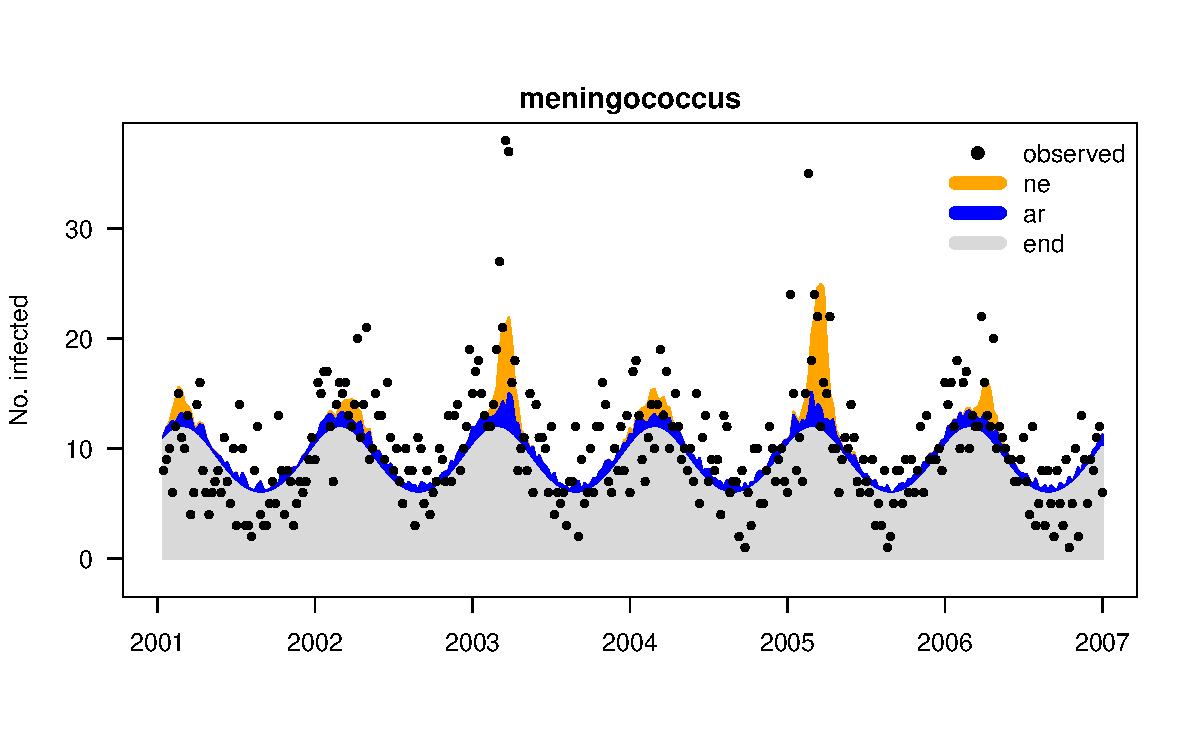
\includegraphics{figs/vignette_hhh4-fit_men}
\end{center}

%%%%%%%%%%%%%%%%%%%%%%%%%%%%%%%%%%%%%%%%%%%%%%%%%%%%%%%%%%%%%%%%%%%%
\subsubsection{Multivariate modelling}
%%%%%%%%%%%%%%%%%%%%%%%%%%%%%%%%%%%%%%%%%%%%%%%%%%%%%%%%%%%%%%%%%%%%

For disease counts observed in a large number of regions, say, (i.e.\
highly multivariate time series of counts) the use of region-specific 
parameters to account for regional heterogeneity is no longer feasible, 
as estimation and identifiability problems may occur. 
\cite{paul-held-2011} propose a random effects formulation to analyze the weekly
number of influenza cases in 140 districts of Southern Germany.
For example, consider a model with random intercepts in the endemic component: 
$c_i \sim \n(0,\sigma^2_\nu), i=1,\ldots,I$.
Such effects are specified in a formula object as
\begin{Schunk}
\begin{Sinput}
> f.end <- ~ -1 + ri(type = "iid", corr = "all")
\end{Sinput}
\end{Schunk}
Setting \code{type = "car"} would assume that the random effects are spatially 
correlated instead of uncorrelated. See \cite{paul-held-2011} for further details.
The argument \code{corr = "all"} allows for correlation between region-specific 
random effects in different components, e.g.\ random incidence levels $c_i$ 
in the endemic component and random effects $b_i$ in the neighbor-driven component.
The following call to \hhh\ fits such a random effects model with
linear trend and $S=3$ seasonal terms in the endemic component and
a fixed autoregressive parameter $\lambda$ to the influenza data 
\citep[cf. model B2 in Tab.~3 in][]{paul-held-2011}.


\begin{Schunk}
\begin{Sinput}
> # weight matrix w_ji = 1/(No. neighbors of j) if j ~ i, and 0 otherwise
> wji <- neighbourhood(flu)/rowSums(neighbourhood(flu))
> # endemic component: iid random effects, linear trend, and S=3 seasonal terms
> f.end <- addSeason2formula(f = ~ -1 + ri(type = "iid", corr="all") + 
+                                 I((t-208)/100), 
+                                 S = 3, 
+                                 period = 52)
> model.B2 <- list(ar = list(f = ~ 1),
+                  ne = list(f = ~ -1+ ri(type = "iid", corr="all"), 
+                            weights = wji),
+                  end = list(f = f.end, offset = population(flu)),
+                  family = "NegBin1"
+                  )
> # fit model
> summary(result.B2 <- hhh4(flu, model.B2))
\end{Sinput}
\end{Schunk}
\begin{Schunk}
\begin{Soutput}
Call: 
hhh4(stsObj = flu, control = model.B2)

Random effects: 
            Var    Corr   
ne.ri(iid)  0.9594        
end.ri(iid) 0.5094 0.5617 

Fixed effects: 
                        Estimates  Std.Error
ar.1                      -0.8976     0.0369
ne.ri(iid)                -1.5256     0.1035
end.I((t - 208)/100)       0.5620     0.0235
end.sin(2 * pi * t/52)     2.1849     0.0985
end.cos(2 * pi * t/52)     2.3319     0.1224
end.sin(4 * pi * t/52)     0.4403     0.1053
end.cos(4 * pi * t/52)    -0.3947     0.0940
end.sin(6 * pi * t/52)     0.3217     0.0648
end.cos(6 * pi * t/52)    -0.2647     0.0631
end.ri(iid)                0.2192     0.1028
1/overdisp                 1.0991     0.0343

penalized log-likelihood:  -18742.42 
marginal log-likelihood:   -343.26 

Number of units:          140 
Number of time points:    416 
\end{Soutput}
\end{Schunk}
Model choice based on information criteria such as AIC or BIC is well
explored and understood for models that correspond to fixed-effects likelihoods.
However, in the presence of random effects their use can be problematic.
For model selection in time series models, the comparison of successive 
one-step-ahead forecasts with the actually observed data 
provides a natural alternative. In this context, \cite{gneiting-raftery-2007}
recommend the use of strictly proper scoring 
rules, such as the logarithmic score or the ranked probability score.
See \cite{czado-etal-2009} and \cite{paul-held-2011} for further details.

One-step-ahead predictions for the last 2 years for model B2 are obtained as 
follows:
\begin{Schunk}
\begin{Sinput}
> pred.B2 <- oneStepAhead(result.B2, tp = nrow(flu) - 2 * 52)
\end{Sinput}
\end{Schunk}
The mean logarithmic and mean ranked probability score are then computed with
\begin{Schunk}
\begin{Sinput}
> colMeans(scores(pred.B2)[, c("logs", "rps")])
\end{Sinput}
\begin{Soutput}
     logs       rps 
0.5632647 0.4362529 
\end{Soutput}
\end{Schunk}


%%%%%%%%%%%%%%%%%%%%%%%%%%%%%%%%%%%%%%%%%%%%%%%%%%%
%% Measles data
As a last example, consider the number of measles cases in the 16 federal states
of Germany, in the years 2005--2007. There is considerable regional variation 
in the incidence pattern which is most likely due to differences in vaccination 
coverage. In the following, information about vaccination coverage in each 
state, namely the log proportion of unvaccinated school starters, is included 
as explanatory variable in a model for the bi-weekly aggregated measles data. 
See \cite{herzog-etal-2010} for further details.

Vaccination coverage levels for the year 2006 are available in the dataset
\code{data(MMRcoverageDE)}. This dataset can be used to compute
the $78\times 16$ matrix \code{vac0} with adjusted
proportions of unvaccinated school starters in each state $i$ used by
\cite{herzog-etal-2010} 
\begin{Schunk}
\begin{Sinput}
> vac0[1:2, 1:5]
\end{Sinput}
\begin{Soutput}
     Baden-Wuerttemberg  Bavaria   Berlin Brandenburg   Bremen
[1,]          0.1000115 0.113261 0.099989   0.0605575 0.115963
[2,]          0.1000115 0.113261 0.099989   0.0605575 0.115963
\end{Soutput}
\end{Schunk}
A Poisson model which links the autoregressive parameter with this covariate
and contains $S=1$ seasonal term in the endemic component 
\citep[cf.~model A0 in Tab.~3 in ][]{herzog-etal-2010} is obtained with
\begin{Schunk}
\begin{Sinput}
> # endemic component: Intercept + S = 1 sine/cosine pair
> f.end <- addSeason2formula(f = ~ 1, S = 1, period = 26)
> # autoregressive component: Intercept + vaccination coverage information
> model.A0 <- list(ar = list(f = ~ 1 + logVac0),
+                  end = list(f = f.end, offset = population(measles2w)),
+                  data = list(t = epoch(measles2w), logVac0 = log(vac0)))
> # fit model
> result.A0 <- hhh4(measles2w, model.A0)    
> # parameter estimates
> round(coef(result.A0, 
+            se = TRUE,              # also return standard errors
+            amplitudeShift = TRUE   # transform sin/cos terms to 
+            ), 2)                   # Amplitude/shift formulation
\end{Sinput}
\begin{Soutput}
                     Estimates Std. Error
ar.1                      3.01       0.52
ar.logVac0                1.38       0.23
end.1                     1.78       0.06
end.A(2 * pi * t/26)      0.66       0.08
end.s(2 * pi * t/26)     -0.10       0.12
\end{Soutput}
\end{Schunk}

%%%%%%%%%%%%%%%%%%%%%%%%%%%%%%%%%%%%%%%%%%%%%%%%%%%%
%% Summary
%%%%%%%%%%%%%%%%%%%%%%%%%%%%%%%%%%%%%%%%%%%%%%%%%%%5
 \section{Summary}
As part of the \R-package \surveillance, the function \hhh\ provides
a flexible tool for the modelling of multivariate time series 
of infectious disease counts. The discussed count data model is able to
account for serial and spatio-temporal correlation, as well as
heterogeneity in incidence levels and disease transmission. 
The functionality of \hhh\ was illustrated using several built-in data 
sets.

\bibliography{references}

\end{document}
 
